\newpage
\section{Scenario 4}\label{sec:scenario4}
The purpose of this scenario is to show what can happen when the UAS loses line-of-sight because of a mountain, as seen on the map in Figure \ref{fig:s4_map}(a). Such that, the UA starts from a visible point (blue circle) and goes behind a mountain, losing LOS (red crosses), but recovers it as seen in \ref{fig:s4_map}(b). Moreover, the controller used in this simulation is a PD controller, such that it reacts fast when field of vision is recovered.

\begin{figure}[H]
	\centering
	\subfigure[UAS Map Positioning]{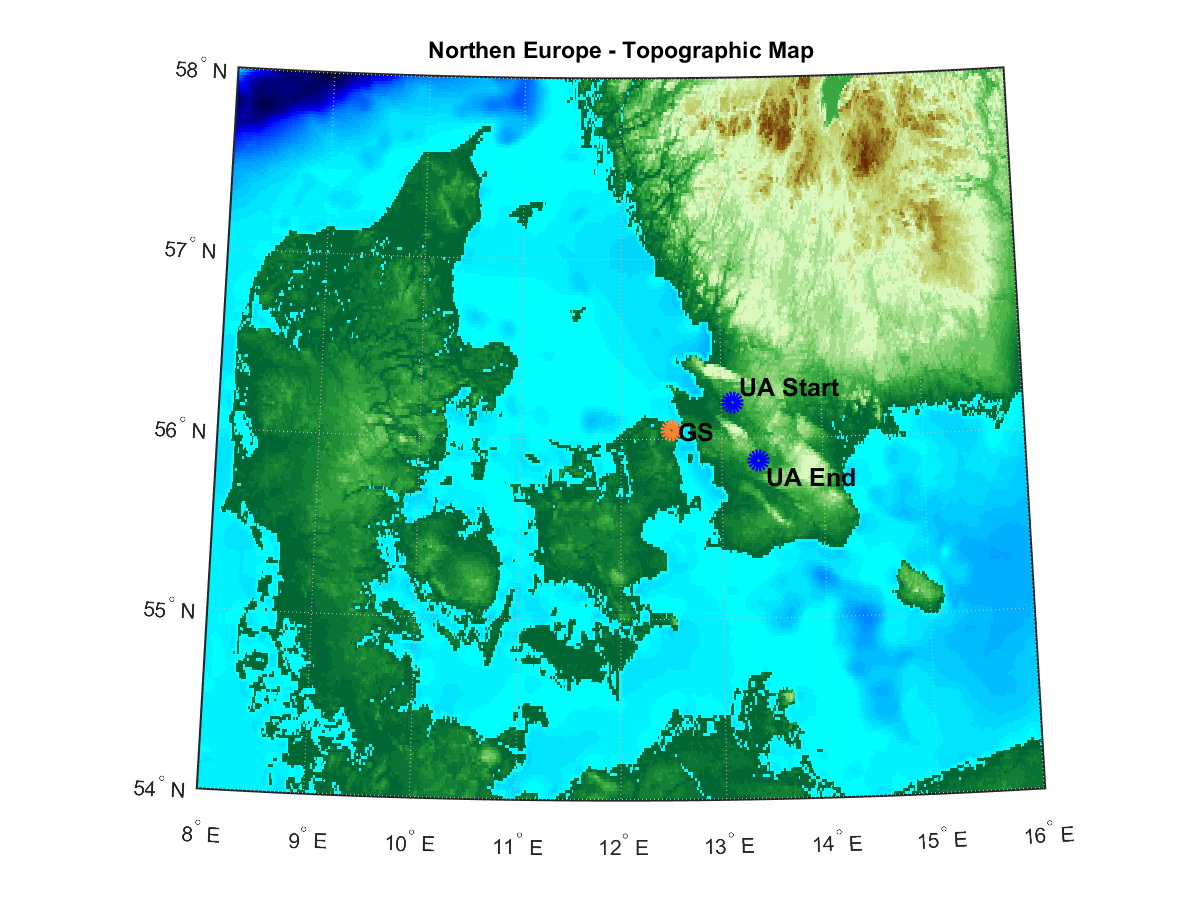
\includegraphics[scale=0.46]{figures/s4_map.png}}
	\\
	\subfigure[LOS and Distance]{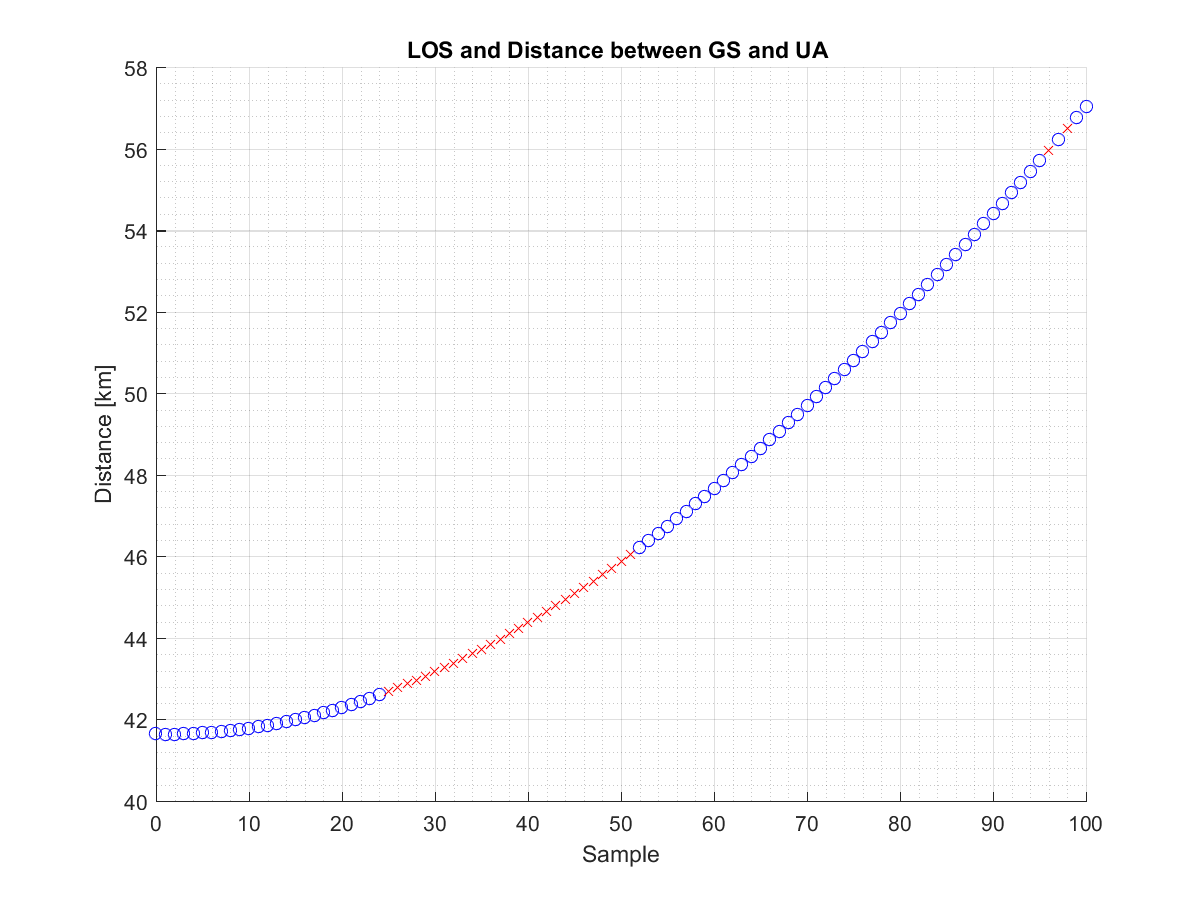
\includegraphics[scale=0.46]{figures/s4_los.png}}
	\caption{Mountain Scenario}
	\label{fig:s4_map}
\end{figure}

\subsection{UA}
In Figure \ref{fig:s4_ua} the angle tracking of the UA antenna can be seen. Thus, in the azimuth angle the optimal angle ($\theta_{OPTIMAL}$) starts at -80$^{\circ}$ and goes to -140$^{\circ}$. Such that, the UA azimuth angle ($\theta_{UA}$) reacts fast with an overshoot of -10$^{\circ}$ and precisely follows the optimal angle. In the case of the elevation angle in the second graph the optimal angle ($\phi_{OPTIMAL}$) is constant for the whole scenario, by reason of the substantial distance between the GS and UA. It can be noticed that in this case the noise can affect the performance of the elevation tracking angle of the aicraft ($\phi_{UA}$) having an error of $\pm3^{\circ}$. 

\begin{figure}[H]
	\centering
	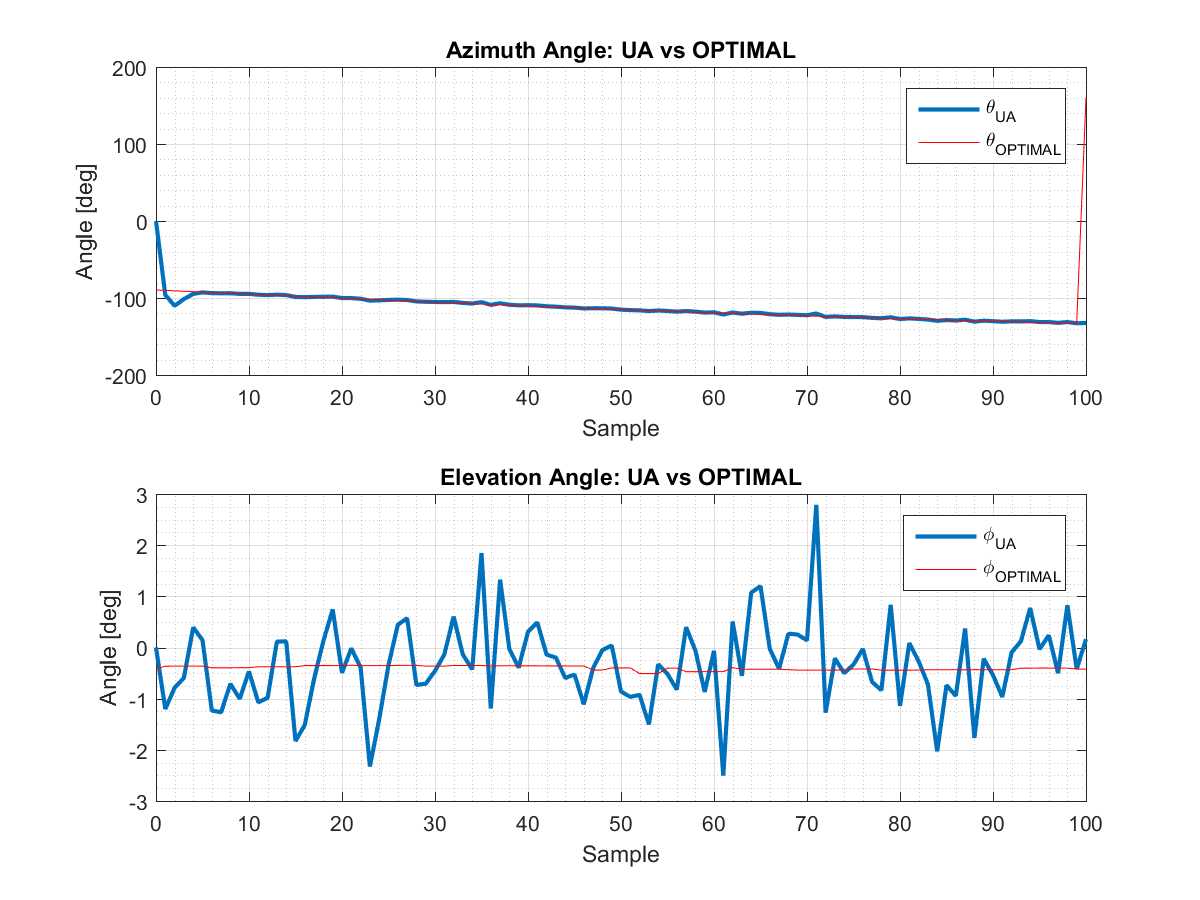
\includegraphics[scale=0.8]{figures/s4_ua.png}
	\caption{Azimuth and elevation angles of UA following the optimal angle}
	\label{fig:s4_ua}
\end{figure}

\subsection{GS}
Looking from the ground station's perspective the angle tracking can be seen in Figure \ref{fig:s4_gs}. Such that, for the azimuth angle of the optimal angle ($\theta_{OPTIMAL}$) starts at 25$^{\circ}$ and goes to -20$^{\circ}$. Such that, the GS azimuth angle ($\theta_{GS}$) reacts rapid with a small overshoot of 2$^{\circ}$ and rigorously follows the optimal angle to the end. In the case of the elevation angle it can be seen that it is similiar as in the case of the UA. Also, the noise affects the performance of the tracking angle of the GS ($\phi_{GS}$), but as a result of using a PD controller the changes are quickly corrected.

\begin{figure}[H]
	\centering
	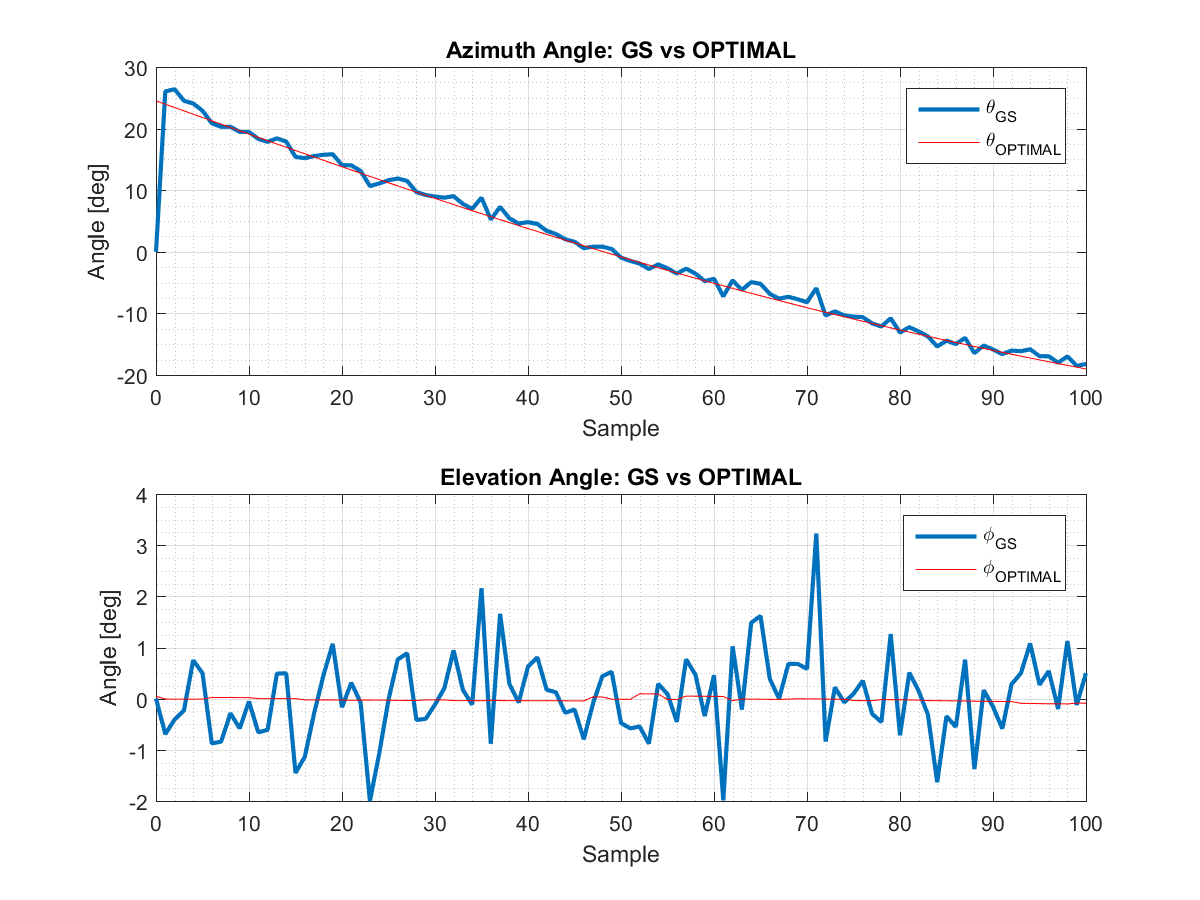
\includegraphics[scale=0.8]{figures/s4_gs.png}
	\caption{Azimuth and elevation angles of GS following the optimal angle}
	\label{fig:s4_gs}
\end{figure}

\subsection{Power}
From the viewpoint of wireless communication, the power at the receiver ($P_{RX}$) antenna at both ends is shown in Figure \ref{fig:s4_power}. Thus, in the beginning there is strong signal, but after losing field of vision (as seen in Figure \ref{fig:s4_map}(b)) the power drops considerably, losing connection. Moreover, there are two spikes of connection loss where LOS is lost at the end due to terrain elevation.

\begin{figure}[H]
	\centering
	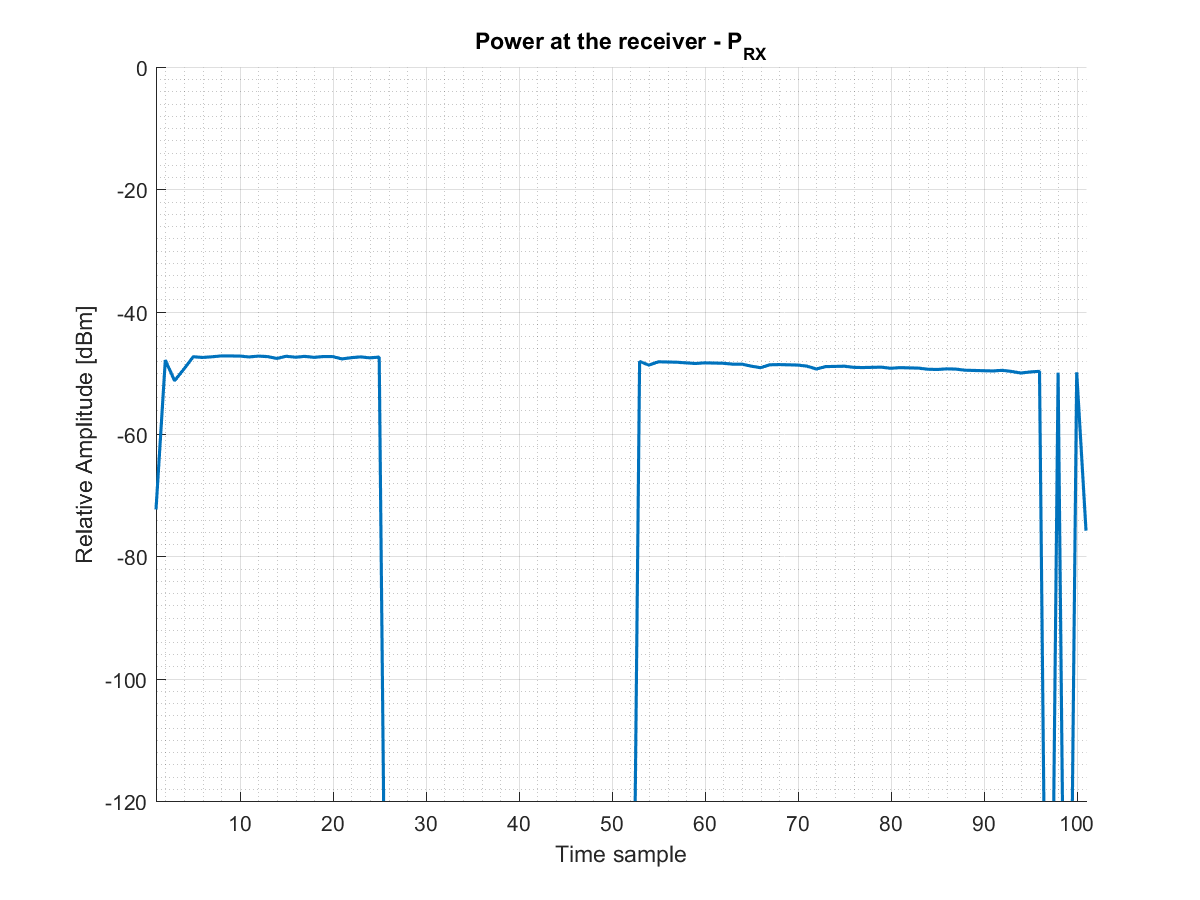
\includegraphics[scale=0.8]{figures/s4_power.png}
	\caption{Power at the receiver's antenna at both ends}
	\label{fig:s4_power}
\end{figure}